\documentclass[11pt,conference,a4paper]{APSIPA2026}
\IEEEoverridecommandlockouts

% --- APSIPA-required page geometry (per official template) ---
\usepackage{geometry}
\geometry{a4paper, top=19mm, bottom=43mm, right=13mm, left=13mm}

% --- Tighter equation spacing (page budget) ---
\setlength{\abovedisplayskip}{4pt}
\setlength{\belowdisplayskip}{4pt}
\setlength{\abovedisplayshortskip}{2pt}
\setlength{\belowdisplayshortskip}{2pt}

% --- APSIPA first-page running header ---
\usepackage{fancyhdr}
\renewcommand{\headrulewidth}{0pt}
\renewcommand{\footrulewidth}{0pt}
\fancypagestyle{firststyle}{
  \fancyhf{}
  \fancyhead[C]{2026 Asia Pacific Signal and Information Processing Association Annual Summit and Conference (APSIPA ASC)}
}
% ============================================================
%  PREAMBLE ADDITIONS — Results & Discussion Chapter

% ============================================================

% --- Tables ---
\usepackage{booktabs}       % \toprule, \midrule, \bottomrule
\usepackage{multirow}       % multi-row table cells
\usepackage{colortbl}       % \rowcolor, \columncolor
\usepackage{xcolor}         % \definecolor, \textcolor

% --- Plots & Figures ---
\usepackage{pgfplots}
\usepackage{pgfplotstable}
\pgfplotsset{compat=1.18}

% --- Symbols ---
\usepackage{pifont}         % \ding{51} = checkmark, \ding{55} = cross

% --- Color palette (used consistently across all figures and tables) ---
\definecolor{clrDS}{RGB}{70,130,180}      % Steel blue: direct supervision
\definecolor{clrV2}{RGB}{205,92,92}       % Coral red: distilled V2-100
\definecolor{clrFT}{RGB}{218,165,32}      % Goldenrod: fine-tuned V2-150
\definecolor{clrMP}{RGB}{150,150,150}     % Gray: MediaPipe SDK
\definecolor{clrTeacher}{RGB}{46,139,87}  % Sea green: teacher reference
\definecolor{clrRowA}{RGB}{245,245,250}   % Light blue-gray: alternating rows
\definecolor{clrHead}{RGB}{230,230,240}   % Slightly darker gray: header rows

% ============================================================
\usepackage{cite}
\usepackage{url}
\usepackage{amsmath,amssymb,amsfonts}
\usepackage{graphicx}
\usepackage{textcomp}
\usepackage{xcolor}
\usepackage{booktabs}
\usepackage{tikz}
\usepackage{pgfplots}
\pgfplotsset{compat=1.18} % Or your specific version
\usetikzlibrary{shapes.geometric, arrows, positioning}

\def\BibTeX{{\rm B\kern-.05em{\sc i\kern-.025em b}\kern-.08em
    T\kern-.1667em\lower.7ex\hbox{E}\kern-.125emX}}

\begin{document}

\title{Heterogeneous Knowledge Distillation for Real-Time 2D Hand Pose Estimation}

\author{
\IEEEauthorblockN{Bea Juliana B. Poquiz$^*$, Rhandley D. Cajote$^*$, and Dale Joshua R. Del Carmen$^*$}
\IEEEauthorblockA{$^*$ Electrical and Electronics Engineering Institute, University of the Philippines Diliman, Quezon City, Philippines\\
E-mail: \{bea.juliana.poquiz, rhandley.cajote, dale.del.carmen\}@eee.upd.edu.ph}
}

\maketitle
\thispagestyle{firststyle}
\pagestyle{empty}

% ============================================================
%  ABSTRACT
% ============================================================
\begin{abstract}
Real-time hand pose estimation underpins a growing range of
human--computer interaction systems, yet leading solutions are either
too heavy for edge deployment or locked inside proprietary,
non-retrainable pipelines such as Google's MediaPipe Hands. This paper
proposes a heterogeneous knowledge distillation framework that
transfers spatial reasoning from a heatmap-based teacher
(HRNetV2-W18 with DARK decoding) to a compact coordinate-regression
student (BlazeHandLandmark) on the Rendered Handpose Dataset (RHD2D).
The output-representation mismatch between heatmaps and coordinates is
resolved by an MSRAHeatmap codec bridge that decodes teacher heatmaps
into sub-pixel coordinate targets at every training iteration,
supervising the student directly in pixel space without modifying
either architecture and without ground-truth labels. The distilled
student attains PCK@0.2\,=\,0.819, AUC\,=\,0.769, and MPJPE\,=\,30.14\,px
on the full RHD2D test set, running at
139\,FPS on an RTX~4050 machine GPU---a 4.8x parameter reduction and
20.2x full-pipeline speedup over the teacher. The complete training
pipeline is open source and retrainable, providing a transparent
alternative to closed hand-tracking systems.
\end{abstract}

\begin{IEEEkeywords}
hand pose estimation, heterogeneous knowledge distillation,
BlazeHand, HRNetV2-W18, real-time inference
\end{IEEEkeywords}

% ============================================================
%  I. INTRODUCTION
% ============================================================
\section{Introduction}

Two-dimensional hand pose estimation -- the localization of 21
anatomical keypoints from a monocular RGB image -- underpins
gesture-based interaction, AR/VR, sign language recognition, and
robotic manipulation~\cite{doosti2019survey,an2025rejshand}.
Google's MediaPipe Hands~\cite{mediapipe2020} dominates real-time
deployment, achieving sub-20\,ms inference on mobile devices through
a lightweight regression-based landmark model. However, its training
data, loss functions, and weights are proprietary and
non-retrainable, so researchers cannot adapt it to specialized
domains such as surgical tracking, industrial safety monitoring, or
domain-specific sign language, where data distributions differ
fundamentally from Google's general-purpose training set.

Knowledge distillation (KD)~\cite{hinton2015distilling} offers a
principled path to an open alternative: train a lightweight student
to mimic a high-capacity teacher, transferring spatial reasoning
without the computational cost. This work applies KD to transfer
knowledge from HRNetV2-W18~\cite{hrnet2019}, a state-of-the-art
heatmap-based teacher achieving PCK@0.2\,=\,0.992 on the RHD2D
benchmark, into a BlazeHandLandmark student. The result is a fully
open and retrainable alternative\footnote{Code:
\url{https://github.com/beapoquiz/heterogeneous-kd-2d-hand-pose-estimation}}
to MediaPipe Hands that any researcher can fine-tune, inspect, and
deploy on domain-specific data without dependence on proprietary
infrastructure.

% ============================================================
%  II. REVIEW OF RELATED WORK
% ============================================================
\section{Review of Related Work}
\label{sec:related}

Two paradigms dominate 2D hand pose estimation from monocular
RGB~\cite{doosti2019survey}. \textbf{Heatmap-based} methods (e.g.,
HRNet~\cite{hrnet2019}) preserve high-resolution spatial
representations, achieving state-of-the-art accuracy at costs that
prohibit real-time edge deployment~\cite{litehrnet2021}.
\textbf{Direct regression} methods predict coordinates
directly~\cite{toshev2014deeppose}, enabling mobile real-time
inference~\cite{howard2017mobilenets} at the cost of the spatial
reasoning needed for occluded-joint localization~\cite{sun2018integral}.

The most widely deployed regression-based solution, MediaPipe
Hands~\cite{mediapipe2020}, combines a BlazePalm detector with a
landmark regression model (1.98\,M parameters, 16.1\,ms on Pixel~3).
Its proprietary pipeline prevents retraining, and its official
evaluation -- palm-size-normalized MSE on a private real-world set
-- leaves generalization to synthetic domains such as
RHD2D~\cite{zimmermann2017learning} uncharacterized.

Bridging this gap requires transferring heatmap-based spatial
precision into a lightweight regressor via knowledge
distillation~\cite{hinton2015distilling}, which raises the problem of
\emph{representation heterogeneity}. Prior work either requires
ground-truth supervision alongside distillation~\cite{sun2018integral}
or addresses only homogeneous regressor-to-regressor
transfer~\cite{saputra2019}, and DARK decoding~\cite{zhang2020dark}
recovers sub-pixel precision from heatmaps but has not been used as a
distillation bridge; fully heterogeneous, ground-truth-free KD from a
heatmap teacher to a regression student for hand pose remains
unaddressed.

% ============================================================
%  III. REPRESENTATION MISMATCH PROBLEM
% ============================================================

\section{Representation Mismatch Problem}
The teacher HRNetV2-W18 (with DARK decoding) outputs spatial heatmaps $(21 \times 64 \times 64)$; the student BlazeHandLandmark regresses coordinate vectors $(21 \times 3)$. No loss applies across the two directly, and the prior work above assumes a shared output representation. This study bridges the mismatch with the MSRAHeatmap codec and second-order Taylor refinement, converting teacher heatmaps into sub-pixel coordinate targets that supervise the student in pixel space -- so the student inherits HRNetV2-W18's spatial calibration without ground-truth labels, and without architectural change to either model.

% ============================================================
%  IV. PROPOSED SOLUTION
% ============================================================
\section{Proposed solution}
\label{sec:method}

\subsection{Framework Overview}

Fig.~\ref{fig:framework} illustrates the proposed heterogeneous KD
pipeline, where a frozen HRNet-W18 teacher generates heatmaps decoded
into sub-pixel coordinate targets that supervise the BlazeHandLandmark
student via a composite Wing\,+\,Bone loss.

\begin{figure}[htbp]
\centering
\resizebox{\columnwidth}{!}{%
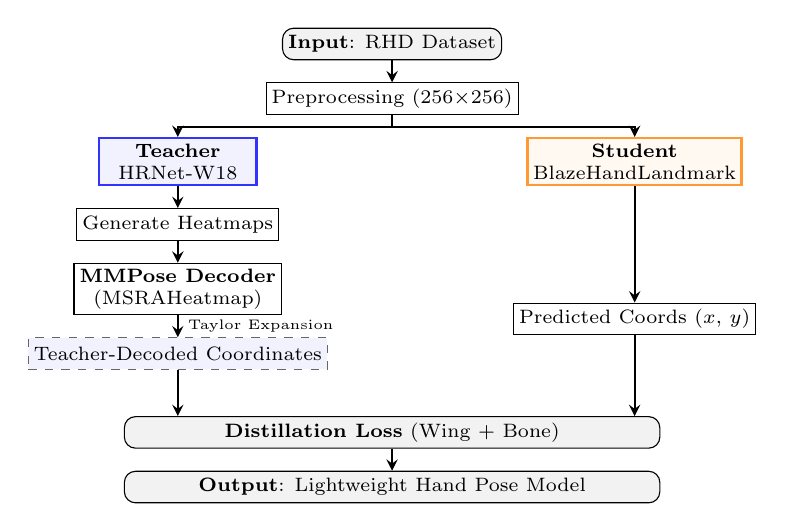
\begin{tikzpicture}[node distance=0.28cm and 0.4cm]
\tikzstyle{startstop} = [rectangle, rounded corners,
    minimum width=2.6cm, minimum height=0.4cm,
    text centered, draw=black, fill=gray!10,
    font=\scriptsize, inner sep=2pt]
\tikzstyle{process} = [rectangle, align=center,
    minimum width=2.0cm, minimum height=0.4cm,
    text centered, draw=black, fill=white,
    font=\scriptsize, inner sep=2pt]
\tikzstyle{teacher} = [rectangle, align=center,
    minimum width=2.0cm, minimum height=0.4cm,
    text centered, draw=blue!80, fill=blue!5,
    line width=0.3mm, font=\scriptsize, inner sep=2pt]
\tikzstyle{student} = [rectangle, align=center,
    minimum width=2.0cm, minimum height=0.4cm,
    text centered, draw=orange!80, fill=orange!5,
    line width=0.3mm, font=\scriptsize, inner sep=2pt]
\tikzstyle{arrow} = [thick,->,>=stealth]

\node (input) [startstop]
    {\textbf{Input}: RHD Dataset};
\node (prep) [process, below=of input]
    {Preprocessing ($256{\times}256$)};
\node (teacher) [teacher, below left=of prep, xshift=0.3cm]
    {\textbf{Teacher}\\HRNet-W18};
\node (student) [student, below right=of prep, xshift=-0.3cm]
    {\textbf{Student}\\BlazeHandLandmark};
\node (heatmaps) [process, below=of teacher]
    {Generate Heatmaps};
\node (decoder) [process, below=of heatmaps]
    {\textbf{MMPose Decoder}\\(MSRAHeatmap)};
\node (targets) [process, below=of decoder,
    fill=blue!5, draw=black!60, dashed]
    {Teacher-Decoded Coordinates};
\node (pred) [process, below=of student, yshift=-1.2cm]
    {Predicted Coords $(x,\,y)$};

% --- FIXED LOSS AND OUTPUT NODES ---
% Centered horizontally with 'prep', positioned vertically below 'targets'
\node (loss) [startstop, minimum width=6.8cm] at ([yshift=-1.0cm]prep |- targets)
    {\textbf{Distillation Loss} (Wing $+$ Bone)};
\node (output) [startstop, below=of loss, minimum width=6.8cm]
    {\textbf{Output}: Lightweight Hand Pose Model};
% -----------------------------------

\draw [arrow] (input) -- (prep);
\draw [arrow] (prep.south) -- ++(0,-0.15cm) -| (teacher.north);
\draw [arrow] (prep.south) -- ++(0,-0.15cm) -| (student.north);
\draw [arrow] (teacher) -- (heatmaps);
\draw [arrow] (heatmaps) -- (decoder);

% --- FIXED LABEL ---
% Changed to a single line to prevent vertical overlap
\draw [arrow] (decoder) -- node[right, font=\tiny]
    {Taylor Expansion} (targets);
% -------------------

% --- FIXED ARROWS TO LOSS BLOCK ---
% Arrows draw straight down from 'targets' and 'pred' to the top edge of 'loss'
\draw [arrow] (targets) -- (loss.north -| targets);
\draw [arrow] (student) -- (pred);
\draw [arrow] (pred) -- (loss.north -| pred);
% ----------------------------------

\draw [arrow] (loss) -- (output);
\end{tikzpicture}%
}
\caption{Heterogeneous KD framework. The teacher (blue) decodes
heatmaps via MSRAHeatmap with Taylor refinement; the student (orange)
directly regresses keypoints.}
\label{fig:framework}
\end{figure}

\subsection{Dataset}

All experiments use the \textbf{Rendered Handpose Dataset (RHD)}~\cite{zimmermann2017learning},
a fully synthetic benchmark rendered from rigged 3D character meshes
under varied viewpoints, poses, and backgrounds, giving pixel-perfect
ground-truth annotations without manual labeling~\cite{hand3d_github}.
Table~\ref{tab:rhd_stats} summarizes its statistics.

\begin{table}[h]
\centering
\caption{RHD Dataset Statistics}
\label{tab:rhd_stats}
\renewcommand{\arraystretch}{0.95}
\begin{tabular}{lc}
\hline
\textbf{Property} & \textbf{Value} \\
\hline
Training samples     & 41,255$^{\dagger}$ \\
Test samples         & 2,727$^{*}$  \\
Native resolution    & $320 \times 320$ px \\
Input resolution     & $256 \times 256$ px \\
Keypoints per image  & 21 \\
Annotation types     & 2D coords, 3D coords, visibility, \\
                     & hand type, segmentation mask, depth \\
\hline
\end{tabular}
\vspace{2pt}
{\scriptsize $^{\dagger}$The raw training folder holds 41,258 images;
3 are absent from \texttt{rhd\_train.json}, the annotation file the
training pipeline loads, and are excluded.
$^{*}$Likewise, 00307.png is absent from the annotation file used by every
evaluation script here -- its ground-truth hand renders almost entirely
off-frame (20 of 21 keypoints) and was dropped during the original dataset
conversion. All PCK/AUC/MPJPE figures in this paper use this 2,727-sample
set.}
\end{table}

Each image is annotated with 21 keypoints: one wrist joint (index~0)
and four joints per finger (Tip--DIP--PIP--MCP, indices~1--20) across
all five digits in thumb/index/middle/ring/pinky
order~\cite{mmpose2020}.

Images are cropped via ground-truth bounding boxes, padded to square,
and resized to $256{\times}256$. Training augmentation includes random
horizontal flip, bounding-box scale/rotate ($\pm180^{\circ}$)/shift,
and photometric distortion. Performance is reported as
\textbf{PCK@0.2} (keypoint within $0.2\times$ bounding-box diagonal)
and \textbf{AUC} (area under the PCK curve)~\cite{zimmermann2017learning}.

\subsection{Distillation Loss}

Let $\hat{\mathbf{p}}\in\mathbb{R}^{21\times 2}$ and
$\mathbf{p}^{T}\in\mathbb{R}^{21\times 2}$ denote the student's
predicted and teacher-decoded keypoint coordinates, respectively.
The total objective is
\begin{equation}
    \mathcal{L} = \mathcal{L}_{\mathrm{wing}} +
    \lambda\,\mathcal{L}_{\mathrm{bone}}, \qquad \lambda=0.002.
    \label{eq:loss}
\end{equation}

\noindent\textbf{Wing Loss}~\cite{wingloss2018} ($w{=}10$,
$\varepsilon{=}2$) is piecewise logarithmic for small residuals and
linear for large ones, providing robustness to outlier joints:
\begin{equation}
    \ell_{\mathrm{wing}}(\delta) =
    \begin{cases}
        w\ln\!\left(1+|\delta|/\varepsilon\right) & |\delta| < w,\\
        |\delta| - C                               & \text{otherwise},
    \end{cases}
    \label{eq:wing}
\end{equation}
where $C = w\bigl(1 - \ln(1+w/\varepsilon)\bigr)$ and
$\delta = \hat{p} - p^{T}$.  The aggregate is the mean over all
joints and coordinate axes:
\begin{equation}
    \mathcal{L}_{\mathrm{wing}} =
    \frac{1}{42N}\sum_{n,k,d}
    \ell_{\mathrm{wing}}\!\left(\hat{p}_{n,k,d}-p^{T}_{n,k,d}\right).
    \label{eq:wing_agg}
\end{equation}

\noindent\textbf{Bone Loss} penalises mean-squared error in predicted
versus teacher bone lengths across the 20 directed segments
$\mathcal{B}$ of the five-finger skeleton (four segments per finger,
all rooted at the wrist):
\begin{equation}
    \mathcal{L}_{\mathrm{bone}} =
    \frac{1}{|\mathcal{B}|N}
    \sum_{(i,j)\in\mathcal{B}}\sum_{n}
    \Bigl(
      \|\hat{\mathbf{p}}_{n,i}-\hat{\mathbf{p}}_{n,j}\|_2
      -
      \|\mathbf{p}^{T}_{n,i}-\mathbf{p}^{T}_{n,j}\|_2
    \Bigr)^{2},
    \label{eq:bone}
\end{equation}

enforcing skeletal consistency independent of absolute joint position.


\subsection{Training Procedure}

The student is trained on RHD in two stages against a frozen HRNet-W18 teacher; Fig.~\ref{fig:training_procedure} gives the full hyperparameter and loss configuration for each. Performance is validated against three baselines: a direct-supervision variant, the teacher itself (upper bound), and the official MediaPipe SDK.

\begin{figure}[htbp]
\centering
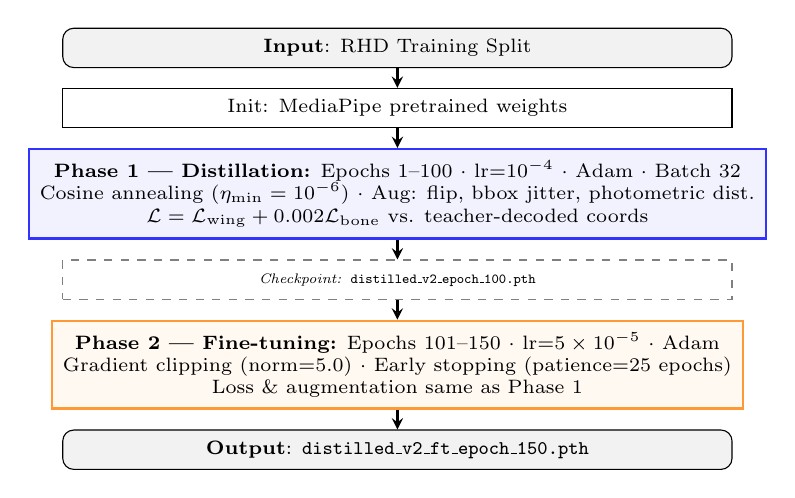
\begin{tikzpicture}[
    % Reduced node distance to save vertical space
    node distance=0.25cm and 0.4cm, 
    % Increased width to 8.5cm and reduced font size to scriptsize for extreme compactness
    base/.style={rectangle, align=center, font=\scriptsize, minimum width=8.5cm},
    startstop/.style={base, rounded corners, minimum height=0.5cm, draw=black, fill=gray!10},
    process/.style={base, minimum height=0.5cm, draw=black, fill=white},
    % Removed hard minimum heights to let boxes shrink
    phase1/.style={base, draw=blue!80, fill=blue!5, line width=0.3mm, inner sep=4pt},
    phase2/.style={base, draw=orange!80, fill=orange!5, line width=0.3mm, inner sep=4pt},
    ckpt/.style={base, draw=black!50, fill=white, dashed, minimum height=0.5cm, font=\tiny},
    arrow/.style={thick,->,>=stealth}
]

%% ── Training Pipeline ────────────────────────────────────────
\node (input) [startstop] {\textbf{Input}: RHD Training Split};

\node (init) [process, below=of input] {Init: MediaPipe pretrained weights};

\node (p1) [phase1, below=of init] {
    \textbf{Phase 1 --- Distillation:} Epochs 1--100 $\cdot$ lr=$10^{-4}$ $\cdot$ Adam $\cdot$ Batch 32\\
    Cosine annealing ($\eta_{\min} = 10^{-6}$) $\cdot$ Aug: flip, bbox jitter, photometric dist.\\
    $\mathcal{L} = \mathcal{L}_{\text{wing}} + 0.002 \mathcal{L}_{\text{bone}}$ vs. teacher-decoded coords
};

\node (ckpt) [ckpt, below=of p1] {\textit{Checkpoint:} \texttt{distilled\_v2\_epoch\_100.pth}};

\node (p2) [phase2, below=of ckpt] {
    \textbf{Phase 2 --- Fine-tuning:} Epochs 101--150 $\cdot$ lr=$5 \times 10^{-5}$ $\cdot$ Adam\\
    Gradient clipping (norm=5.0) $\cdot$ Early stopping (patience=25 epochs)\\
    Loss \& augmentation same as Phase 1
};

\node (output) [startstop, below=of p2] {\textbf{Output}: \texttt{distilled\_v2\_ft\_epoch\_150.pth}};

%% ── Main arrows ─────────────────────────────────────────────
\draw [arrow] (input) -- (init);
\draw [arrow] (init) -- (p1);
\draw [arrow] (p1) -- (ckpt);
\draw [arrow] (ckpt) -- (p2);
\draw [arrow] (p2) -- (output);

\end{tikzpicture}
\caption{Streamlined training procedure flowchart.}
\label{fig:training_procedure}
\end{figure}

%============================================================
%  V. RESULTS AND DISCUSSION  (revised — tightened, reordered)
%  Thesis: 2D Hand Pose Estimation via Knowledge Distillation
%  Student: BlazeHandLandmark  |  Teacher: HRNetV2-W18 + DARK
%  Dataset: RHD2D (41,255 train / 2,727 test)
% ===========================================================

\section{Experimental Results}
\label{sec:results}

% ── §5.1 Evaluation Protocol ────────────────────────────────
\subsection{Evaluation Protocol}
\label{sec:eval_protocol}

All experiments run on an NVIDIA RTX~4050 Laptop GPU (CUDA~12.1,
PyTorch~2.1.0) over the full RHD2D test split (2,727 images, 21
keypoints/hand). Three accuracy metrics are reported: PCK@0.2
(keypoint within $\tau = 0.2 \times 256 = 51.2$\,px of GT), AUC (area
under the PCK curve over 20 thresholds in $[0,\,128]$\,px), and
MPJPE (mean Euclidean distance in pixels), with GPU inference speed
(FPS) as the efficiency metric. All trained models are evaluated
identically: affine-cropped $256{\times}256$ inputs, fixed GT
bounding boxes, the same 2,727-sample split.

Two MediaPipe-related references are kept distinct. The
\textbf{official MediaPipe Hands SDK} (\texttt{mediapipe} pip
package, closed weights) is a domain-gap reference, not a trained
competitor: it was trained on real-world and photorealistic imagery,
not RHD2D's flat-shaded synthetic style~\cite{mediapipe2020}, so any
score gap reflects a \emph{domain gap}, not an architectural limit.
The \textbf{BlazeHandLandmark student} was instead initialized from
the \textbf{zmurez MediaPipePyTorch port}~\cite{mediapipepytorch2021},
an open reimplementation with converted weights, which separates the
architecture's own starting point from the SDK's out-of-domain
performance.

Detection failure is defined per system. For the SDK, its BlazePalm
detector and landmark model jointly return no hand. For the zmurez
weights and the distilled student -- which never call BlazePalm and
run directly on the fixed $256{\times}256$ crop -- the model's own
\texttt{hand\_flag} head scores $\leq0.5$. Failures are scored, not
excluded: every keypoint on a failed frame gets a worst-case
256\,px error. That is more conservative than published MediaPipe
benchmarks, which score detected frames only. Scored separately, the
SDK detects 66.2\% of frames (PCK@0.2\,=\,0.901 detected-only) and the
zmurez weights 80.1\% (0.783); both localize much better than their
all-frames figures suggest.

% ── §5.2 Experimental Setup and Training Behavior ───────────
% MERGED §5.2 (V1 vs V2) + §5.3 (Training Convergence)
% Both were single-paragraph subsections describing training-side
% design and behavior, so they belong together.
\subsection{Experimental Setup and Training Behavior}
\label{sec:setup_training}

Table~\ref{tab:v1v2} summarises the V2 design changes that address
the overfitting and instability seen in V1. V2 is the configuration
evaluated in the rest of this paper. Figure~\ref{fig:learning_curves} shows V2 validation metrics
over 100 distillation epochs, scored against teacher-decoded
coordinates on a 200-sample RHD subset every 5 epochs. PCK@0.2 peaks
at epoch~65 (0.769) and settles 0.0017 lower by epoch~100 (0.768),
while AUC and MPJPE improve monotonically through epoch~100;
epoch~100 is therefore taken as the Stage~1 checkpoint, since the
model keeps refining spatial calibration after coarse-threshold
accuracy saturates.

\begin{table}[!t]
\caption{Design Differences: Distillation V1 vs.\ V2}
\label{tab:v1v2}
\centering
\footnotesize
\setlength{\tabcolsep}{4pt}
\renewcommand{\arraystretch}{1.0}
\begin{tabular}{lll}
\toprule
\textbf{Component} & \textbf{V1} & \textbf{V2} \\
\midrule
Student init.      & Random            & MediaPipe-inspired pretrained \\
Augmentation       & None              & Flip+Scale+Rotate+Color \\
Loss               & MSE               & Wing+Bone ($\lambda$=0.002) \\
LR schedule        & Fixed $10^{-4}$   & Cosine $10^{-4}\!\to\!10^{-6}$ \\
Validation         & None              & PCK+MPJPE every 5\,ep. \\
Coord.\ clipping   & No                & $[0,255]$ \\
Grad.\ clipping    & No                & $\|\nabla\|_{\max}=5.0$ (FT) \\
Epochs             & 210               & 100 distil.\ + 50 fine-tune \\
\bottomrule
\end{tabular}
\end{table}

\begin{figure}[!t]
\centering
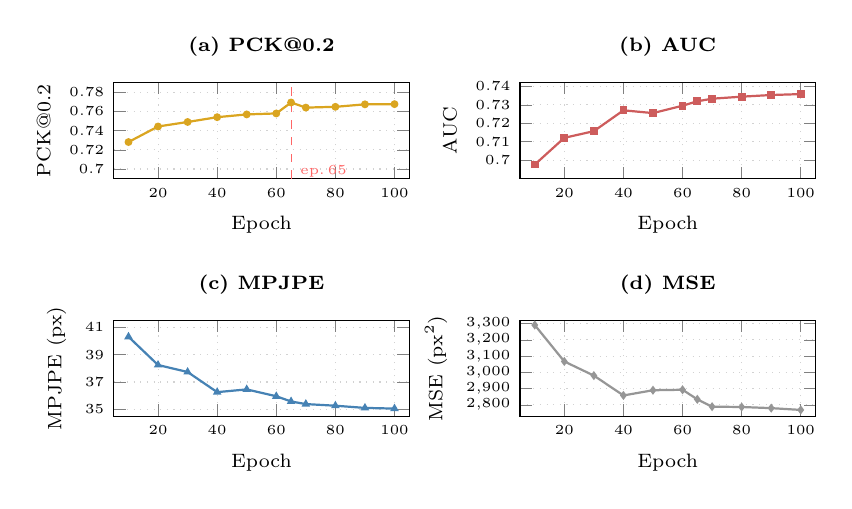
\begin{tikzpicture}
% ---- panel (a) PCK ----
\begin{axis}[
  name=ax1,
  width=0.44\columnwidth, height=2.8cm,
  xlabel={\scriptsize Epoch},
  ylabel={\scriptsize PCK@0.2},
  xlabel style={font=\scriptsize},
  ylabel style={font=\scriptsize},
  tick label style={font=\tiny},
  ymin=0.69, ymax=0.79,
  xmin=5, xmax=105,
  xtick={20,40,60,80,100},
  ytick={0.70,0.72,0.74,0.76,0.78},
  grid=major, grid style={dotted,gray!35},
  title={\scriptsize\bfseries (a) PCK@0.2},
  title style={font=\scriptsize},
]
\addplot[color=clrFT, thick, mark=*, mark size=1pt] coordinates {
  (10,0.7281)(20,0.7443)(30,0.7490)(40,0.7540)
  (50,0.7569)(60,0.7579)(65,0.7693)(70,0.7640)
  (80,0.7648)(90,0.7674)(100,0.7676)
};
\addplot[dashed, color=red!60, very thin] coordinates {(65,0.69)(65,0.79)};
\node[font=\tiny, color=red!60] at (axis cs:76,0.697) {ep.\,65};
\end{axis}

% ---- panel (b) AUC ----
\begin{axis}[
  name=ax2,
  at={(ax1.north east)}, xshift=40pt, % Increased xshift to prevent horizontal overlap
  anchor=north west,
  width=0.44\columnwidth, height=2.8cm,
  xlabel={\scriptsize Epoch},
  ylabel={\scriptsize AUC},
  xlabel style={font=\scriptsize},
  ylabel style={font=\scriptsize},
  tick label style={font=\tiny},
  ymin=0.690, ymax=0.742,
  xmin=5, xmax=105,
  xtick={20,40,60,80,100},
  ytick={0.70,0.71,0.72,0.73,0.74},
  grid=major, grid style={dotted,gray!35},
  title={\scriptsize\bfseries (b) AUC},
  title style={font=\scriptsize},
]
\addplot[color=clrV2, thick, mark=square*, mark size=1pt] coordinates {
  (10,0.6976)(20,0.7121)(30,0.7157)(40,0.7270)
  (50,0.7255)(60,0.7295)(65,0.7319)(70,0.7333)
  (80,0.7344)(90,0.7353)(100,0.7358)
};
\end{axis}

% ---- panel (c) MPJPE ----
\begin{axis}[
  name=ax3,
  at={(ax1.south west)}, yshift=-1.8cm, % Increased negative yshift to prevent vertical overlap
  anchor=north west,
  width=0.44\columnwidth, height=2.8cm,
  xlabel={\scriptsize Epoch},
  ylabel={\scriptsize MPJPE (px)},
  xlabel style={font=\scriptsize},
  ylabel style={font=\scriptsize},
  tick label style={font=\tiny},
  ymin=34.5, ymax=41.5,
  xmin=5, xmax=105,
  xtick={20,40,60,80,100},
  ytick={35,37,39,41},
  grid=major, grid style={dotted,gray!35},
  title={\scriptsize\bfseries (c) MPJPE},
  title style={font=\scriptsize},
]
\addplot[color=clrDS, thick, mark=triangle*, mark size=1pt] coordinates {
  (10,40.30)(20,38.24)(30,37.73)(40,36.26)
  (50,36.46)(60,35.96)(65,35.58)(70,35.39)
  (80,35.27)(90,35.11)(100,35.06)
};
\end{axis}

% ---- panel (d) MSE ----
\begin{axis}[
  name=ax4,
  at={(ax3.north east)}, xshift=40pt, % Increased xshift to prevent horizontal overlap
  anchor=north west,
  width=0.44\columnwidth, height=2.8cm,
  xlabel={\scriptsize Epoch},
  ylabel={\scriptsize MSE (px$^{2}$)},
  xlabel style={font=\scriptsize},
  ylabel style={font=\scriptsize},
  tick label style={font=\tiny},
  ymin=2730, ymax=3320,
  xmin=5, xmax=105,
  xtick={20,40,60,80,100},
  ytick={2800,2900,3000,3100,3200,3300},
  grid=major, grid style={dotted,gray!35},
  title={\scriptsize\bfseries (d) MSE},
  title style={font=\scriptsize},
]
\addplot[color=clrMP, thick, mark=diamond*, mark size=1pt] coordinates {
  (10,3291)(20,3067)(30,2980)(40,2858)
  (50,2890)(60,2893)(65,2834)(70,2789)
  (80,2787)(90,2780)(100,2769)
};
\end{axis}
\end{tikzpicture}
\caption{Distillation V2 validation metrics over 100 epochs.
PCK@0.2 peaks at epoch~65 while AUC and MPJPE continue improving
through epoch~100.}
\label{fig:learning_curves}
\end{figure}

% ── §5.3 Quantitative Results ───────────────────────────────
% FLATTENED: removed \subsubsection* nesting; both tables now sit
% under a single subsection with transition prose between them.
\subsection{Quantitative Results}
\label{sec:quant}

Table~\ref{tab:trained} reports all models trained or fine-tuned on
RHD2D, evaluated on the full 2,727-sample test set against GT
annotations. Two Direct Sup.\ baselines appear in this paper: the
\emph{parity baseline}, a corrected, parity-controlled retrain
described below, and the \emph{original baseline}, an earlier,
uncorrected version mentioned only where explicitly noted, for
comparison.

The parity baseline (protocol v2match) is the direct-supervision result used in the headline comparison. It reaches PCK@0.2 = 0.970, AUC = 0.894, and MPJPE = 13.63 px, ahead of both distilled models by 12.6–12.7 pp AUC. AUC integrates PCK over thresholds as tight as about 6.7 px, so this gap holds at fine spatial precision, not just in the lenient 51.2 px PCK@0.2 window. This baseline shares its training recipe with the distillation runs (Table~\ref{tab:v1v2}): the same coordinate frame and the same Wing + Bone loss combination. The per-joint breakdown (Table~\ref{tab:perjoint}) reports this same parity baseline, joint by joint. Direct supervision leading the comparison follows from the teacher's own accuracy ceiling: the teacher itself reaches only AUC = 0.902 against ground truth, so a distilled student inherits the teacher's error on top of its own, while direct supervision only has its own error to overcome. Distillation's usual advantage — learning efficiently from scarce labeled data — does not apply here, since RHD2D's synthetic labels are pixel-perfect and available for every sample. That said, the parity baseline's recipe is inherited unchanged from the distillation configuration rather than tuned for direct supervision on its own, so this result reflects direct supervision under a distillation-derived recipe, not its best achievable setting. The parity baseline shows no overfitting through epoch 100: the epoch-90 checkpoint scores within 0.01 pp AUC of the final one. Within the distillation arm, Stage 2 fine-tuning adds a modest gain over Stage 1 ($+$0.002 AUC, $-$0.21 px MPJPE, with PCK@0.2 statistically tied), showing Phase 1 already captures most of the transferable knowledge, with fine-tuning mainly refining convergence. The teacher remains the accuracy upper bound at AUC = 0.902, but at 6.9 FPS it is not a deployment candidate.

\begin{table}[!t]
\caption{Trained Model Comparison --- Full RHD2D Test Set
         (2,727 samples, vs.\ GT annotations)}
\label{tab:trained}
\centering
\renewcommand{\arraystretch}{0.95}
\resizebox{\columnwidth}{!}{%
\begin{tabular}{lccccccc}
\toprule
\textbf{Model} & \textbf{Params} & \textbf{PCK@0.2} & \textbf{AUC}
  & \textbf{MPJPE} & \textbf{Det.}$^{c}$ & \textbf{GPU} & \textbf{$\Delta$ AUC} \\
 & \textbf{(M)} & & & \textbf{(px)} & \textbf{Rate} & \textbf{FPS} & \textbf{vs.\ Direct} \\
\midrule
Direct Sup.\ (parity, ep.\,100)$^{d}$
  & 2.01 & 0.970 & 0.894 & 13.63 & 100\% & 139.0 & ref. \\
Stage 1: Dist.\ V2 (ep.\,100)
  & 2.01 & 0.819 & 0.767 & 30.35 & 100\%   & 139.0 & $-$0.127 \\
Stage 2: FT V2 (ep.\,150)
  & 2.01 & 0.819$^{b}$ & 0.769
  & 30.14 & 100\% & 139.0 & $-$0.126 \\
\midrule
Teacher (HRNetV2-W18)$^{a}$
  & 9.64 & 0.992 & 0.902 & 2.18 & 100\% & 6.9 & --- \\
\bottomrule
\multicolumn{8}{l}{\scriptsize $^{a}$Own-protocol reference (mmpose
  \texttt{Runner.test()}); bbox-relative PCK threshold, not}\\
\multicolumn{8}{l}{\scriptsize the fixed 51.2\,px used above -- not
  deployment-comparable. $^{b}$Statistically tied with}\\
\multicolumn{8}{l}{\scriptsize Dist.\ V2-100 on PCK@0.2 (0.8190 vs.\
  0.8188 unrounded; single-run, no seed}\\
\multicolumn{8}{l}{\scriptsize variance); best of the two
  distilled configurations on AUC/MPJPE.}\\
\multicolumn{8}{l}{\scriptsize $^{c}$Not evidence of detection
  capability: \texttt{hand\_flag} is never trained by any loss}\\
\multicolumn{8}{l}{\scriptsize term (see Quantitative Results), for all rows shown.}\\
\multicolumn{8}{l}{\scriptsize $^{d}$Corrected parity retrain
  (v2match); supersedes an earlier, buggy implementation}\\
\multicolumn{8}{l}{\scriptsize (PCK\,=\,0.425, AUC\,=\,0.538,
  MPJPE\,=\,59.87\,px) that read targets from an uncorrected}\\
\multicolumn{8}{l}{\scriptsize coordinate frame -- see
  Quantitative Results.}
\end{tabular}%
}
\end{table}

Two starting states of the same architecture, both scored against GT
on the full test set, put the pipeline's contribution in context.
Random weights score PCK@0.2\,=\,0.001, AUC\,=\,0.014,
MPJPE\,=\,188.88\,px at 0.00\% detection. The zmurez
BlazeHandLandmark weights~\cite{mediapipepytorch2021} -- taken
before distillation, with no ground truth or teacher signal, and
distinct from the official SDK in Table~\ref{tab:consolidated} (see
Evaluation Protocol) -- score 0.627, 0.589, 78.25\,px, 80.05\%. The
rise from PCK@0.2\,=\,0.627 to 0.819 after distillation
(Table~\ref{tab:trained}, FT~V2 ep.\,150) measures what the
framework adds to localization accuracy. The rise in detection rate
(80.05\%\,$\to$\,100\%) is \emph{not} part of that gain, and we
withdraw it as a claimed strength. Tracing the training code shows
that \texttt{hand\_flag} never appears in any loss term, so its
weights get no gradient update while the backbone is heavily
retrained by the coordinate-regression objective. What is left is a
frozen classification head reading features it was never
recalibrated for: a number that is correct but says nothing about
detection ability. The zmurez row's 80.05\% comes from the same code
path and does discriminate, so the metric itself is sound; only the
fine-tuned checkpoint's head has lost its signal. One caveat applies
to the localization gain itself. All three trained-model rows were
trained and evaluated on BGR-ordered pixels, an inherited OpenCV
default, while the zmurez and SDK rows were correctly RGB-converted,
so an unquantified channel-order confound accompanies the
distillation effect. These results are not a critique of MediaPipe
Hands or the zmurez port on their intended domain; they isolate the
domain-adaptation problem that this open, retrainable framework
addresses.

% ── §5.4 Efficiency ─────────────────────────────────────────
\subsection{Efficiency and Real-Time Performance}
\label{sec:efficiency}

The fine-tuned student is $4.8{\times}$ smaller than the HRNetV2-W18
teacher in both parameters and weight size, and runs at 139.0\,FPS on
GPU---a $20.2{\times}$ full-pipeline speedup and $4.6{\times}$ above
the 30\,FPS real-time threshold. CPU throughput (25.6\,FPS median)
falls just below threshold, the primary limitation on CPU-only edge
devices. Batch throughput scales near-linearly to batch~8
(892\,img/s) before plateauing at batch~16 (905\,img/s), confirming
efficient GPU use for batched video pipelines
(Table~\ref{tab:throughput}). MediaPipe Hands Full's reported
5.3--16.1\,ms on Pixel~3/S20/iPhone~11~\cite{mediapipe2020} is not
comparable here, but it does indicate that the BlazeHandLandmark
architecture suits mobile deployment.

\begin{table}[!t]
\caption{Multi-Batch GPU Throughput --- Student (FT V2 ep.\,150)}
\label{tab:throughput}
\centering
\footnotesize
\setlength{\tabcolsep}{8pt}
\renewcommand{\arraystretch}{0.92}
\begin{tabular}{cc}
\toprule
\textbf{Batch Size} & \textbf{Throughput (img/s)} \\
\midrule
1  & 126.3 \\
4  & 473.1 \\
8  & 891.9 \\
16 & 905.1 \\
\bottomrule
\end{tabular}
\end{table}

% ── §5.5 Qualitative and Per-Joint Results ──────────────────
\subsection{Qualitative and Per-Joint Results}
\label{sec:perjoint}

Table~\ref{tab:perjoint} reports per-joint PCK@0.2 for the three
trained models, now including the parity baseline's own per-joint
breakdown. The result confirms the aggregate finding in Quantitative
Results at finer detail: the parity baseline wins all 21 of 21
joints against both distilled models, by a wide margin (parity
scores range 0.93--0.99; the two distilled models range 0.68--0.90).
This is not a separate result -- it follows directly from the same
12.6--12.7\,pp AUC gap already reported above.

A different pattern holds within the distilled models themselves:
Tip is the lowest-scoring joint of every finger, and the average
scores go Tip (0.742) $<$ DIP (0.816) $<$ PIP (0.836) $<$ MCP
(0.875) for FT~V2-150, with Dist.\ V2-100 in the same order. One
possible reason is that the teacher network is less confident about
some joints than others, but we have not tested it: the code needed
to check is not currently available, so we do not claim to know the
real cause. A different explanation, such as how each
joint naturally moves or how the loss function weights each joint,
is also possible, but confirming it needs a proper, saved analysis.

\begin{table}[!t]
\caption{Per-Joint PCK@0.2 --- Trained Models (RHD2D, vs.\ GT)}
\label{tab:perjoint}
\centering
\scriptsize
\setlength{\tabcolsep}{2.2pt}
\renewcommand{\arraystretch}{0.92}
\resizebox{\columnwidth}{!}{%
\begin{tabular}{lcccc@{\hskip 5pt}cccc@{\hskip 5pt}cccc}
\toprule
& \multicolumn{4}{c}{\textbf{Direct Sup.}$^{*}$}
& \multicolumn{4}{c}{\textbf{Dist.\ V2-100}}
& \multicolumn{4}{c}{\textbf{FT V2-150}} \\
\cmidrule(lr){2-5}\cmidrule(lr){6-9}\cmidrule(lr){10-13}
\textbf{Digit} & MCP & PIP & DIP & Tip & MCP & PIP & DIP & Tip
               & MCP & PIP & DIP & Tip \\
\midrule
Thumb  & 0.986 & 0.973 & 0.961 & 0.932
       & 0.899 & 0.836 & 0.819 & 0.762
       & 0.897 & 0.835 & 0.821 & 0.766 \\
Index  & 0.984 & 0.985 & 0.975 & 0.949
       & 0.902 & 0.854 & 0.805 & 0.745
       & 0.897 & 0.848 & 0.806 & 0.747 \\
Middle & 0.992 & 0.988 & 0.983 & 0.958
       & 0.908 & 0.879 & 0.838 & 0.786
       & 0.906 & 0.879 & 0.840 & 0.781 \\
Ring   & 0.981 & 0.981 & 0.979 & 0.938
       & 0.883 & 0.863 & 0.844 & 0.728
       & 0.884 & 0.859 & 0.845 & 0.730 \\
Pinky  & 0.967 & 0.966 & 0.958 & 0.939
       & 0.790 & 0.762 & 0.768 & 0.681
       & 0.790 & 0.763 & 0.768 & 0.685 \\
\midrule
Wrist  & \multicolumn{4}{c}{0.985}
       & \multicolumn{4}{c}{0.847}
       & \multicolumn{4}{c}{0.850} \\
Mean   & \multicolumn{4}{c}{0.970}
       & \multicolumn{4}{c}{0.819}
       & \multicolumn{4}{c}{0.819} \\
Range  & \multicolumn{4}{c}{0.061}
       & \multicolumn{4}{c}{0.227}
       & \multicolumn{4}{c}{0.221} \\
\bottomrule
\multicolumn{13}{l}{\scriptsize Direct Sup.\ (parity) leads all 21/21 joints; between the distilled}\\
\multicolumn{13}{l}{\scriptsize models, FT~V2-150 leads 12/21 and Dist.\ V2-100 leads 9/21 (GT}\\
\multicolumn{13}{l}{\scriptsize annotations, uniform coord.\ space, see Evaluation Protocol). Mean and}\\
\multicolumn{13}{l}{\scriptsize range (max$-$min) are over all 21 joints.}\\
\multicolumn{13}{l}{\scriptsize $^{*}$Corrected parity retrain (v2match), matching Table~\ref{tab:trained}$^{d}$;}\\
\multicolumn{13}{l}{\scriptsize per-joint breakdown computed separately from the aggregate retrain.}
\end{tabular}%
}
\end{table}

% --- Fig. 4 (per-joint PCK@0.2 bar chart) removed for page budget
% (page-cut pass, cut 4). It visualized the same 21x3 values already
% tabulated exactly in Table VII (tab:perjoint) immediately above,
% and the proximal-to-distal gradient / direct-supervision variability
% pattern it showed is already stated in prose in this subsection and
% in Section V-H.3 (Per-Joint Structural Patterns). Not cross-referenced
% elsewhere (verified via grep before removal). Do not reintroduce
% without reconsidering the page budget.

For space, teacher-vs.-student skeleton overlays on RHD2D test
samples and a live webcam demonstration on real, out-of-distribution
input are provided in the code repository linked in the Introduction.
Both match the pattern above: overlay deviations cluster at Tip
joints, and webcam inference stays stable without domain-specific
adaptation.

% ── §5.7 Consolidated Comparison ────────────────────────────
\subsection{Consolidated Model Comparison}
\label{sec:summary_table}

Table~\ref{tab:consolidated} consolidates accuracy, efficiency,
and open-source trainability for all models considered in this
study.

\begin{table}[!t]
\caption{Consolidated Model Comparison}
\label{tab:consolidated}
\centering
\renewcommand{\arraystretch}{0.92}
\resizebox{\columnwidth}{!}{%
\begin{tabular}{lccccc}
\toprule
\textbf{Criterion} & \textbf{MP SDK} & \textbf{Teacher} & \textbf{Direct} & \textbf{Dist.} & \textbf{FT V2} \\
                   &                 & \textbf{HRNetV2} & \textbf{Sup.}$^{f}$   & \textbf{V2-100} & \textbf{-150} \\
\midrule
Params.         & 1.98M & 9.64M  & 2.01M & 2.01M & 2.01M \\
GPU FPS         & ---$^{c}$ & 6.9    & 139   & 139   & 139   \\
PCK@0.2$^{a}$   & 0.597 & 0.992$^{b}$ & 0.970 & 0.819 & 0.819 \\
AUC$^{a}$       & 0.553 & 0.902$^{b}$ & 0.894 & 0.767 & 0.769 \\
MPJPE$^{a}$ (px)& 100.75 & 2.18$^{b}$  & 13.63 & 30.35 & 30.14 \\
Det.\ rate$^{d}$ & 66.23\%& 100\%$^{b}$  & 100\%&100\% & 100\% \\
RT/Open/KD$^{e}$ & Y/N/N & N/Y/-- & Y/Y/N & Y/Y/Y & Y/Y/Y \\
\bottomrule
\end{tabular}%
}

\vspace{3pt}
\parbox{\columnwidth}{\scriptsize $^{a}$All-frames scoring, fixed 51.2\,px
  threshold, full 2,727-sample test set (see Evaluation Protocol); the MP~SDK row is a
  single reconciled run, superseding a retired 500-sample result.
  $^{b}$Own-protocol reference (mmpose \texttt{Runner.test()}),
  bbox-relative PCK threshold -- not comparable to the fixed
  51.2\,px used elsewhere; Det.\ rate undefined (no confidence head),
  shown as 100\% by convention. $^{c}$Mobile GPU
  5.3--16.1\,ms~\cite{mediapipe2020}; not comparable to RTX~4050.
  $^{d}$For Direct/Dist./FT~V2 only: \texttt{hand\_flag} is never
  trained by any loss term (see Quantitative Results), so 100\% is not
  evidence of detection capability. MP~SDK's 66.23\% is a genuine
  BlazePalm result; the teacher's is undefined (footnote~$b$).
  $^{e}$RT~=~real-time at $\geq$30\,FPS on evaluated hardware
  (footnote~$c$; teacher 6.9\,FPS, below threshold);
  Open~=~open-source/retrainable; KD~=~knowledge-distillation
  supervision (`--'\,=\,n/a to a teacher). $^{f}$Corrected parity
  retrain (v2match); see Table~\ref{tab:trained}$^{d}$ and
  Quantitative Results.}
\end{table}

% ============================================================
%  VI. CONCLUSIONS AND RECOMMENDATIONS
% ============================================================
\section{Conclusions and Recommendations}
\label{sec:conclusion}

This work proposed and validated a heterogeneous knowledge
distillation framework bridging a heatmap-based teacher
(HRNetV2-W18 with DARK decoding) and a regression-based student
(BlazeHandLandmark) via MSRAHeatmap codec decoding, meeting the
problem statement's three objectives. First, the bridge transfers
the spatial reasoning of a teacher nearly $5\times$ larger and
$20\times$ slower into a student that stays deployable at real-time
speeds. Second, retraining through this pipeline yields an
open alternative to MediaPipe Hands reaching $\text{PCK@0.2} = 0.819$ on
the RHD2D synthetic domain, up from $0.627$ at the pre-distillation
starting point, on inputs where the SDK is out of domain. Third,
under an identical, distillation-derived recipe, direct supervision
outperforms the framework by $12.6\text{--}12.7\,\text{pp}$ AUC once the earlier
baseline's coordinate-frame bug and missing regularization term are
corrected (see Quantitative Results). The advantage previously
reported for distillation came from an incomplete baseline, not from
the supervision signal itself. On this fully-labeled synthetic
benchmark, the framework's value therefore lies in compressing the teacher $4.8\times$ into a real-time
student without using ground-truth labels, not in exceeding a
well-trained direct-supervision baseline.

Per-joint results confirm this holds at fine detail, not just on
average: the parity baseline wins all 21 of 21 joints against both
distilled models. Within the distilled models themselves, a separate
pattern remains unexplained -- Tip is consistently their
lowest-scoring joint, MCP their highest -- motivating the kinematic
and loss-weighting directions below.

More importantly, this study has already met its main goal:
an open, retrainable alternative to MediaPipe Hands now exists.
Real-hand generalization is already observed, not just hoped for:
run live via webcam (\texttt{webcam\_demo\_finetuned.py}), it tracks
real hands in real time under ordinary indoor lighting, despite
training entirely on RHD2D's synthetic renders -- which strong
RHD2D scores alone do not guarantee. A quantitative check agrees: a
zero-shot test of the RHD-trained FT~V2-150 checkpoint on 1,628 real
FreiHAND samples, with no fine-tuning, reaches $\text{PCK@0.2} = 0.757$,
$\text{AUC} = 0.719$, and $\text{MPJPE} = 36.0\,\text{px}$. The useful next step is not
testing whether the model works on real hands, but improving how
well it does, via fuller evaluation on FreiHAND, OneHand10K, and
HO-3D.

% ============================================================
%  REFERENCES
% ============================================================
\scriptsize
\begin{thebibliography}{00}

\bibitem{doosti2019survey}
B.~Doosti, ``Hand pose estimation: A survey,''
arXiv:1903.01013, 2019.

\bibitem{an2025rejshand}
S.~An et al.,
``ReJSHand: Efficient real-time hand pose estimation and mesh reconstruction
using refined joint and skeleton features,''
arXiv:2503.05995, 2025.

\bibitem{hrnet2019}
K.~Sun, B.~Xiao, D.~Liu, and J.~Wang,
``Deep high-resolution representation learning for human pose estimation,''
in \textit{Proc.\ IEEE/CVF CVPR}, 2019, pp.~5693--5703.

\bibitem{litehrnet2021}
Y.~Yu et al.,
``Lite-HRNet: A lightweight high-resolution network,''
in \textit{Proc.\ IEEE/CVF CVPR}, 2021, pp.~10440--10450.

\bibitem{toshev2014deeppose}
A.~Toshev and C.~Szegedy,
``DeepPose: Human pose estimation via deep neural networks,''
in \textit{Proc.\ IEEE/CVF CVPR}, 2014, pp.~1653--1660.

\bibitem{howard2017mobilenets}
A.~G.~Howard et al.,
``MobileNets: Efficient convolutional neural networks for mobile vision applications,''
arXiv:1704.04861, 2017.

\bibitem{sun2018integral}
X.~Sun et al.,
``Integral human pose regression,''
in \textit{Proc.\ ECCV}, 2018, pp.~529--545.

\bibitem{mediapipe2020}
F.~Zhang et al.,
``MediaPipe Hands: On-device real-time hand tracking,''
arXiv:2006.10214, 2020.

\bibitem{mediapipepytorch2021}
Z.~Murez et al.,
``MediaPipePyTorch,'' GitHub, 2021. [Online].
Available: \url{https://github.com/zmurez/MediaPipePyTorch}

\bibitem{zimmermann2017learning}
C.~Zimmermann and T.~Brox,
``Learning to estimate 3D hand pose from single RGB images,''
in \textit{Proc.\ IEEE/CVF ICCV}, 2017, pp.~4903--4911.

\bibitem{hand3d_github}
C.~Zimmermann,
``hand3d,'' GitHub, 2017. [Online].
Available: \url{https://github.com/lmb-freiburg/hand3d}

\bibitem{hinton2015distilling}
G.~Hinton, O.~Vinyals, and J.~Dean,
``Distilling the knowledge in a neural network,''
arXiv:1503.02531, 2015.

\bibitem{zhang2020dark}
F.~Zhang et al.,
``Distribution-aware coordinate representation for human pose estimation,''
in \textit{Proc.\ IEEE/CVF CVPR}, 2020, pp.~7093--7102.

\bibitem{saputra2019}
M.~R.~U.~Saputra et al.,
``Distilling knowledge from a deep pose regressor network,''
in \textit{Proc.\ IEEE/CVF ICCV}, 2019, pp.~263--272.

\bibitem{mmpose2020}
MMPose Contributors,
``OpenMMLab pose estimation toolbox and benchmark,''
GitHub, 2020. [Online].
Available: \url{https://github.com/open-mmlab/mmpose}

\bibitem{wingloss2018}
Z.~Feng et al.,
``Wing loss for robust facial landmark localisation with CNNs,''
in \textit{Proc.\ IEEE/CVF CVPR}, 2018, pp.~2235--2245.

\end{thebibliography}

\end{document}
